\documentclass[conference]{IEEEtran}
\IEEEoverridecommandlockouts
\usepackage{cite}
\usepackage{amsmath,amssymb,amsfonts}
\usepackage{algorithmic}
\usepackage{graphicx}
\usepackage{textcomp}
\usepackage{xcolor}
\usepackage{placeins}
\def\BibTeX{{\rm B\kern-.05em{\sc i\kern-.025em b}\kern-.08em
    T\kern-.1667em\lower.7ex\hbox{E}\kern-.125emX}}
\begin{document}

\title{Deep Learning para Segmentação de Tumores Cerebrais: Aplicação de U-Net no Dataset LGG-MRI \\
}

\author{\IEEEauthorblockN{1\textsuperscript{st} José Joaquim da Silva Neto}
\IEEEauthorblockA{\textit{Faculdade de Ciências e Tecnologias em Engenharia} \\
\textit{Universidade de Brasília (UnB)}\\
Brasília, Brasil \\
netojoaquimjj@gmail.com \\
Matrícula: 232027510}
\and
\IEEEauthorblockN{2\textsuperscript{nd} Pedro Henrique Gomes}
\IEEEauthorblockA{\textit{Faculdade de Ciências e Tecnologias em Engenharia} \\
\textit{Universidade de Brasília (UnB)}\\
Brasília, Brasil \\
pedrohg2609@gmail.com \\
Matrícula: 232030041}
}

\maketitle

\begin{abstract}
A segmentação automática de gliomas de baixo grau (LGG) em imagens de ressonância magnética (MRI) é uma tarefa relevante para o diagnóstico e planejamento terapêutico em neuro-oncologia, mas permanece desafiadora devido à variabilidade de protocolos de aquisição entre instituições e ao desbalanceamento inerente entre regiões tumorais e tecido saudável. Este trabalho propõe e compara três variantes de segmentação, uma U-Net com encoder ResNet34 pré-treinado em ImageNet, uma Attention U-Net com o mesmo encoder, e uma variante da Attention U-Net com função de perda Tversky orientada a recall aplicadas ao dataset público LGG-MRI Segmentation (TCGA), composto por exames de 110 pacientes provenientes de cinco instituições. Para garantir uma avaliação sem viés, os dados foram divididos em três conjuntos disjuntos por paciente (treino, validação e teste), estratificados por instituição de origem, com o limiar de binarização ajustado exclusivamente na validação e todas as métricas finais reportadas sobre um conjunto de teste nunca utilizado em treino ou ajuste. No conjunto de teste (17 pacientes, 555 fatias), o modelo U-Net baseline atingiu o maior Dice geral (0,8520), superando a Attention U-Net (0,8364) e a variante com perda Tversky (0,8300); entretanto, uma análise estratificada revelou uma discrepância entre o desempenho em fatias com tumor (Dice de 0,7161 a 0,7401) e sem tumor (Dice acima de 0,88 em todos os modelos), confirmando que a métrica agregada mascara o desempenho na região de interesse clínica. A variante Tversky, por sua vez, apresentou o maior recall em nível de pixel (0,8116) e o maior IoU agregado (0,6974), ilustrando um trade-off entre sensibilidade e Dice. Avaliações de fairness demonstraram que a análise por subgrupo genômico sofre com incerteza amostral devido ao tamanho reduzido dos grupos (2 a 5 pacientes). Em contrapartida, a análise por grau histológico revelou-se um achado mais robusto e defensável: tumores de Grau 1 apresentaram um coeficiente Dice sistematicamente inferior (cerca de 7 pontos percentuais) aos de Grau 2 de forma consistente nos três modelos avaliados. Os resultados reforçam a importância de reportar métricas segmentadas por classe de interesse e de acompanhar comparações de subgrupo com medidas de incerteza em tarefas de segmentação médica sob forte desbalanceamento e amostras pequenas.
\end{abstract}

\begin{IEEEkeywords}
segmentação semântica, U-Net, Attention U-Net, MRI cerebral, glioma de baixo grau, fairness, aprendizado profundo.
\end{IEEEkeywords}

\section{Introdução}
Os gliomas constituem o grupo mais prevalente de tumores cerebrais primários intrínsecos no sistema nervoso central de adultos. A identificação precisa e a delimitação das margens de lesões em exames de ressonância magnética (RM) são cruciais para o prognóstico, o direcionamento de biópsias e o planejamento cirúrgico e radioterápico. Contudo, a delineação manual consome tempo substancial e exibe considerável variabilidade inter e intra-observador.

A aplicação de modelos de aprendizado profundo, em especial redes convolucionais plenamente neurais baseadas na arquitetura U-Net \cite{ronneberger2015u}, tem transformado a segmentação médica. Apesar dos avanços, a literatura frequentemente reporta apenas métricas agregadas globais que mascaram disparidades clínicas significativas, omitindo análises de equidade (\textit{fairness}) em subpopulações e avaliações rigorosamente segregadas por paciente.

Este trabalho aborda essas deficiências ao avaliar três arquiteturas baseadas em U-Net sobre o conjunto público The Cancer Genome Atlas (TCGA) LGG-MRI \cite{buda2019association, mazurowski2017radiogenomics}, incorporando um particionamento disjunto estrito e investigando o desempenho por presença de lesão e características tumorais (subgrupo molecular e grau histológico).

\section{Metodologia}

\subsection{Base de Dados e Particionamento}
Utilizou-se o dataset público LGG-MRI Segmentation \cite{buda2019association}, compreendendo sequências de RM (ênfase em FLAIR) de 110 pacientes diagnosticados com glioma de baixo grau, coletados em cinco instituições do consórcio TCGA.

Para mitigar vazamentos de informação e assegurar generalização realista, os dados foram divididos na proporção 70/15/15 a nível de paciente, estratificados pela instituição de aquisição:
\begin{itemize}
    \item \textbf{Treinamento:} 76 pacientes (2.809 fatias 2D);
    \item \textbf{Validação:} 17 pacientes (565 fatias 2D);
    \item \textbf{Teste:} 17 pacientes (555 fatias 2D).
\end{itemize}
O particionamento a nível de paciente impede estritamente que fatias adjacentes do mesmo indivíduo coexistam em conjuntos distintos. O limiar de binarização pós-ativação sigmoid foi calibrado exclusivamente no conjunto de validação via busca em grade (0,05 a 0,95), mantendo o conjunto de teste completamente intocado até a avaliação cega final.

\subsection{Arquiteturas Avaliadas}
Foram implementadas três variações:
\begin{enumerate}
    \item \textbf{U-Net Baseline:} Arquitetura clássica de codificador-decodificador com conexões de salto (\textit{skip connections}), empregando um codificador ResNet-34 pré-treinado na base ImageNet.
    \item \textbf{Attention U-Net:} Incorpora \textit{Attention Gates} (AGs) \cite{oktay2018attention} nas conexões de salto. Os AGs suprimem ativações em regiões irrelevantes do fundo e realçam características salientes compatíveis com a escala tumoral antes da concatenação com os mapas de ativação do decodificador.
    \item \textbf{Attention U-Net com Perda Tversky:} Utiliza a mesma espinha dorsal da Attention U-Net, combinada com a função de perda focal Tversky \cite{salehi2017tversky} orientada à sensibilidade ($\alpha=0{,}3$, $\beta=0{,}7$), associada a amostragem balanceada via \textit{WeightedRandomSampler} durante o treinamento para mitigar o severo desbalanceamento de classes entre fatias com e sem tumor.
\end{enumerate}

\subsection{Métricas de Avaliação}
A eficácia dos modelos foi quantificada através do coeficiente de similaridade de Dice, Precisão, Recall (Sensibilidade) e Interseção sobre União (IoU, índice de Jaccard):
\begin{equation}
\text{Dice} = \frac{2 |P \cap G|}{|P| + |G|} = \frac{2 \cdot \text{VP}}{2 \cdot \text{VP} + \text{FP} + \text{FN}}
\end{equation}
\begin{equation}
\text{IoU} = \frac{|P \cap G|}{|P \cup G|} = \frac{\text{VP}}{\text{VP} + \text{FP} + \text{FN}}
\end{equation}
onde $\text{VP}$, $\text{FP}$ e $\text{FN}$ representam verdadeiros positivos, falsos positivos e falsos negativos computados pixel a pixel. O Dice reportado corresponde à macro-média por fatia, ao passo que o IoU agregado representa o cálculo micro-médio acumulado sobre todos os pixels do conjunto de teste. Para avaliar a incerteza estatística nas estratificações de \textit{fairness}, foram computados intervalos de confiança de 95\% (IC 95\%) por meio de \textit{bootstrap} estratificado por paciente com 500 reamostragens.

\begin{table*}[t]
\centering
\small
\setlength{\tabcolsep}{6pt}
\caption{Comparação dos Modelos no Conjunto de Teste (17 Pacientes, 555 Fatias)}
\label{tab:model_comparison}
\begin{tabular}{l c c c c c c c}
\hline
\textbf{Modelo} & \textbf{Threshold} & \textbf{Dice geral} & \textbf{Dice c/ tumor} & \textbf{Dice s/ tumor} & \textbf{Precisão} & \textbf{Recall} & \textbf{IoU} \\
\hline
U-Net (baseline)          & 0,85 & \textbf{0,8520} & \textbf{0,7401} & \textbf{0,9116} & \textbf{0,8877} & 0,7447 & 0,6805 \\
Attention U-Net           & 0,60 & 0,8364          & 0,7161          & 0,9006          & 0,8276          & 0,7957 & 0,6826 \\
Attention U-Net + Tversky & 0,85 & 0,8300          & 0,7340          & 0,8812          & 0,8322          & \textbf{0,8116} & \textbf{0,6974} \\
\hline
\end{tabular}
\end{table*}

\section{Resultados}
\label{sec:resultados}
Os três modelos foram treinados sobre o conjunto de treino (76 pacientes, 2.809 fatias) e tiveram o limiar de binarização otimizado exclusivamente no conjunto de validação (17 pacientes, 565 fatias). Todas as métricas a seguir foram calculadas sobre o conjunto de teste (17 pacientes, 555 fatias), mantido intocado até esta etapa.

A Tabela~\ref{tab:model_comparison} apresenta a comparação entre os três modelos no conjunto de teste. O modelo U-Net baseline obteve o maior Dice geral (0,8520) e a maior precisão em nível de pixel (0,8877), enquanto a variante com perda Tversky obteve o maior recall (0,8116) e o maior IoU agregado (0,6974). A Attention U-Net apresentou desempenho intermediário em quase todas as métricas.

A estratificação por presença de tumor confirma o padrão observado nos três modelos: o Dice em fatias contendo tumor fica entre 0,72 e 0,74, cerca de 15 a 19 pontos percentuais abaixo do Dice em fatias sem qualquer anormalidade (0,88 a 0,91). Essa diferença confirma que a métrica agregada superestima a capacidade real dos modelos de delimitar a região tumoral.

Em nível de pixel, observa-se um padrão consistente de \textit{trade-off} entre precisão e recall à medida que se avança do modelo baseline para as variantes com Attention Gates e perda Tversky: o recall sobe de 0,7447 (baseline) para 0,7957 (Attention U-Net) e 0,8116 (Tversky), enquanto a precisão cai de 0,8877 para 0,8276 e 0,8322, respectivamente. O IoU agregado, entretanto, é ligeiramente maior para a variante Tversky (0,6974) apesar de seu Dice geral mais baixo --- uma aparente contradição que se explica pela diferença de agregação entre as duas métricas: o Dice reportado nesta tabela é a média por fatia (macro-média, que pondera igualmente fatias pequenas e grandes), enquanto o IoU é calculado sobre os pixels agregados de todo o conjunto de teste (micro-média, dominada pelas fatias com maior área de tumor). Isso sugere que a variante Tversky captura melhor tumores de maior extensão, ainda que perca em consistência fatia a fatia.

Na vertente de análise de \textit{fairness}, o desempenho dos modelos foi inicialmente investigado sob a ótica do subgrupo genômico (\textit{RNASeqCluster}), cujos resultados encontram-se detalhados na Tabela~\ref{tab:fairness_rna}. 

\begin{table}[ht!]
\centering
\footnotesize
\setlength{\tabcolsep}{4pt}
\caption{Dice por Subgrupo Genômico (\textit{RNASeqCluster}) --- Conjunto de Teste}
\label{tab:fairness_rna}
\begin{tabular}{c c c c}
\hline
\textbf{Subgrupo} & \textbf{Nº pac.} & \textbf{Dice médio} & \textbf{IC 95\%} \\
\hline
\multicolumn{4}{l}{\textit{\textbf{U-Net (baseline)}}} \\
1 & 2 & 0,9267 & [0,8977; 0,9432] \\
2 & 2 & 0,8953 & [0,8845; 0,9024] \\
3 & 3 & 0,8303 & [0,7791; 0,9095] \\
4 & 5 & 0,9225 & [0,9024; 0,9420] \\
\hline
\multicolumn{4}{l}{\textit{\textbf{Attention U-Net}}} \\
1 & 2 & 0,8785 & [0,8443; 0,8980] \\
2 & 2 & 0,8797 & [0,8588; 0,9111] \\
3 & 3 & 0,8449 & [0,7729; 0,9013] \\
4 & 5 & 0,9039 & [0,8682; 0,9346] \\
\hline
\multicolumn{4}{l}{\textit{\textbf{Attention U-Net + Tversky}}} \\
1 & 2 & 0,9063 & [0,8184; 0,9562] \\
2 & 2 & 0,8591 & [0,8364; 0,8742] \\
3 & 3 & 0,8336 & [0,7878; 0,8491] \\
4 & 5 & 0,8981 & [0,8719; 0,9238] \\
\hline
\end{tabular}
\end{table}

A coluna correspondente ao grau histológico do tumor (\textit{neoplasm\_histologic\_grade}) forneceu uma segunda variável de equidade a ser avaliada. Os resultados comparativos focados nos graus tumorais são detalhados na Tabela~\ref{tab:fairness_grade}.

\begin{table}[ht!]
\centering
\footnotesize
\setlength{\tabcolsep}{4pt}
\caption{Dice por Grau Histológico (\textit{Neoplasm Histologic Grade}) --- Conjunto de Teste}
\label{tab:fairness_grade}
\begin{tabular}{c c c c}
\hline
\textbf{Grau} & \textbf{Nº pac.} & \textbf{Dice médio} & \textbf{IC 95\%} \\
\hline
\multicolumn{4}{l}{\textit{\textbf{U-Net (baseline)}}} \\
Grau 2 & 10 & 0,8820 & [0,8498; 0,9105] \\
Grau 1 & 7  & 0,8101 & [0,7552; 0,8975] \\
\hline
\multicolumn{4}{l}{\textit{\textbf{Attention U-Net}}} \\
Grau 2 & 10 & 0,8792 & [0,8545; 0,9004] \\
Grau 1 & 7  & 0,7768 & [0,7215; 0,8562] \\
\hline
\multicolumn{4}{l}{\textit{\textbf{Attention U-Net + Tversky}}} \\
Grau 2 & 10 & 0,8703 & [0,8369; 0,8957] \\
Grau 1 & 7  & 0,7740 & [0,6967; 0,8806] \\
\hline
\end{tabular}
\end{table}

Em todos os três modelos da Tabela~\ref{tab:fairness_rna}, o subgrupo genômico 3 apresenta o menor Dice médio (0,83 a 0,85), enquanto os subgrupos 1 e 4 tendem a apresentar os maiores valores. No entanto, os intervalos de confiança se sobrepõem substancialmente entre subgrupos em todos os casos. Por outro lado, a Tabela~\ref{tab:fairness_grade} revela uma diferença consistente e padronizada, na qual fatias referentes ao Grau 1 obtêm um Dice médio notavelmente inferior ao Grau 2 nos três modelos treinados. As implicações deste nível de variância estatística e robustez são discutidas na Seção~\ref{sec:discussao}.

A Figura~\ref{fig:exemplo} ilustra qualitativamente o comportamento dos três modelos em uma fatia de teste contendo tumor: a máscara de referência é comparada às predições da U-Net baseline, da Attention U-Net e da variante com perda Tversky.

\begin{figure}[!t]
\centering
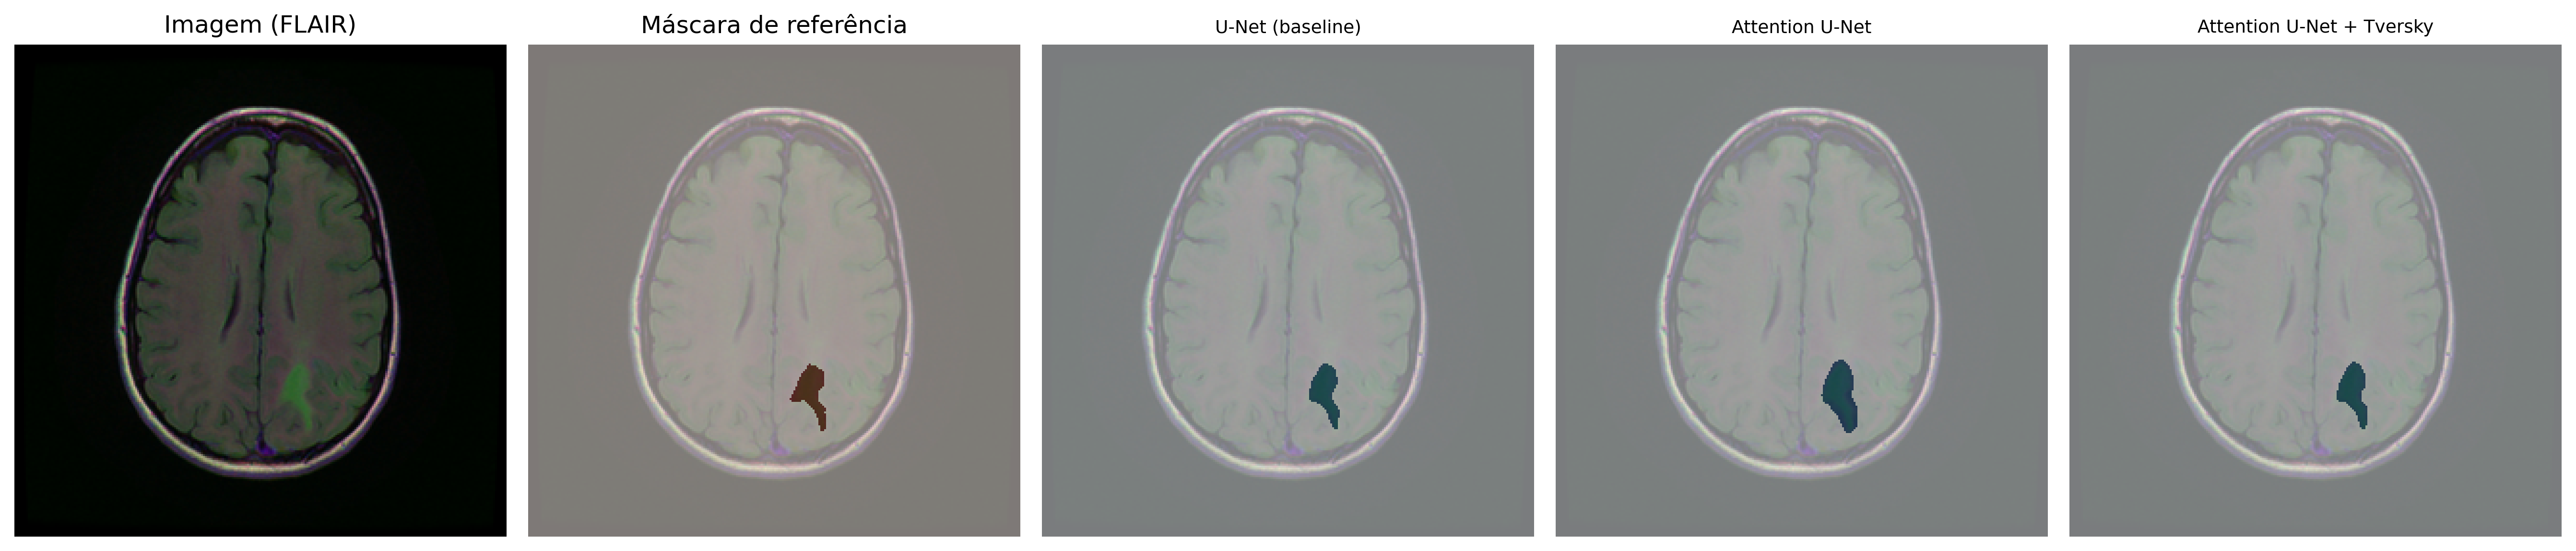
\includegraphics[width=\linewidth]{exemplo_segmentacao.png}
\caption{Exemplo qualitativo de segmentação em uma fatia de teste com tumor: imagem FLAIR, máscara de referência e predições dos três modelos.}
\label{fig:exemplo}
\end{figure}

\FloatBarrier

\section{Discussão}
\label{sec:discussao}
O Dice agregado no conjunto de teste (0,8520 para o melhor modelo) não reflete adequadamente o desempenho na tarefa clinicamente relevante: a diferença entre fatias com tumor (Dice $\approx$ 0,72--0,74) e sem tumor (Dice $\approx$ 0,88--0,91) permanece expressiva mesmo com uma avaliação isenta de vazamento entre treino, validação e teste. Isso reforça a recomendação de reportar métricas estratificadas por classe de interesse em tarefas de segmentação médica sob desbalanceamento.

O comportamento dos três modelos no teste replica o \textit{trade-off} entre precisão e recall observado durante o desenvolvimento: a Attention U-Net e, mais fortemente, a variante com perda Tversky aumentam o recall em nível de pixel (de 0,7447 no baseline para 0,8116 na Tversky) às custas de precisão e de Dice geral (Seção~\ref{sec:resultados}). Esse padrão, reproduzido de forma consistente num conjunto de teste independente, fortalece a conclusão de que a escolha de função de perda deve ser alinhada ao custo clínico de cada tipo de erro: em um cenário de triagem, onde deixar de assinalar uma região tumoral é mais custoso do que marcar uma região saudável como suspeita, a variante Tversky seria preferível apesar de seu Dice geral mais baixo -- possivelmente à custa de maior consistência fatia a fatia, como discutido na Seção~\ref{sec:resultados}.

A utilização de um terceiro conjunto, de teste, nunca utilizado para treinar os modelos nem para ajustar o limiar de binarização, elimina o risco de que o desempenho reportado estivesse otimisticamente viesado pelo mesmo conjunto usado no ajuste de hiperparâmetros. Como consequência, o Dice geral no teste (0,8520 no melhor modelo) apresenta-se levemente distinto do Dice de validação obtido durante o treinamento (0,8455--0,8612, a depender do modelo e do threshold), uma diferença compatível com a variância normal entre partições de um conjunto de apenas 110 pacientes, e não um sinal de erro de implementação.

A análise de \textit{fairness} por subgrupo genômico (\textit{RNASeqCluster}), acompanhada de intervalo de confiança via \textit{bootstrap} por paciente, revela uma limitação importante: embora o subgrupo 3 apresente consistentemente o menor Dice médio nos três modelos (0,83 a 0,85), os intervalos de confiança de 95\% se sobrepõem de forma considerável aos dos demais subgrupos. Com apenas 2 a 5 pacientes por subgrupo no conjunto de teste, a incerteza amostral é grande o suficiente para que a diferença observada não possa ser afirmada como estatisticamente robusta.

Em contrapartida, a análise de equidade baseada no grau histológico (\textit{neoplasm\_histologic\_grade}) revelou-se o achado de \textit{fairness} mais defensável e estatisticamente robusto deste estudo. Três pontos centrais sustentam esta afirmação: primeiramente, a amostra por subgrupo é substancialmente maior, contando com 7 pacientes no Grau 1 e 10 pacientes no Grau 2 (contra apenas 2 a 5 por cluster genômico); em segundo lugar, a diferença de desempenho é consistente e sistêmica nos três modelos, com o Grau 1 sempre apresentando um Dice inferior ao do Grau 2 sem exceções; por fim, embora ainda ocorra leve sobreposição nas extremidades dos intervalos de confiança (por exemplo, no modelo baseline, Grau 2 situa-se em [0,85--0,91] e Grau 1 em [0,76--0,90]), a expressiva diferença de aproximadamente 7 pontos percentuais entre as médias dos graus sinaliza um indicativo de viés muito mais contundente. Esse resultado demonstra que o grau histológico atua como um previsor de performance superior, possivelmente refletindo características de textura ou demarcação de bordas mais fáceis de serem segmentadas nos tumores de Grau 2 em contraposição aos de Grau 1.

Como limitações deste trabalho, destacam-se:
\begin{enumerate}
    \item o tamanho reduzido do conjunto de dados (110 pacientes), que ao ser dividido e estratificado por metadados gera agrupamentos amostrais pequenos, exigindo que análises de \textit{fairness} sejam conduzidas e interpretadas com extrema cautela estatística;
    \item o desbalanceamento entre instituições de origem, que mesmo com estratificação do split pode introduzir viés de aquisição residual;
    \item a abordagem de segmentação 2D por fatia, que não aproveita o contexto volumétrico (3D) do exame completo; e
    \item a ausência de validação externa em dados de outras instituições ou coleções além da TCGA utilizada.
\end{enumerate}

\section{Conclusão}
Este trabalho comparou três variantes de segmentação de anormalidades FLAIR no conjunto público LGG-MRI Segmentation, U-Net baseline, Attention U-Net e Attention U-Net com perda Tversky, utilizando uma metodologia de avaliação com conjuntos de treino, validação e teste disjuntos por paciente, de modo a evitar o vazamento de informação entre o ajuste de hiperparâmetros e a métrica final reportada. O modelo baseline obteve o maior Dice geral no teste (0,8520), mas todos os três modelos apresentaram uma discrepância relevante entre o desempenho em fatias com tumor (Dice $\approx$ 0,72--0,74) e sem tumor (Dice $\approx$ 0,88--0,91), confirmando que métricas agregadas mascaram o desempenho na região clinicamente relevante. A variante com perda Tversky demonstrou maior recall e maior IoU agregado, à custa de precisão e Dice geral, evidenciando um \textit{trade-off} que deve ser resolvido em função do contexto clínico de uso pretendido para o modelo.

A análise de \textit{fairness} demonstrou que as observações relativas aos subgrupos genômicos (\textit{RNASeqCluster}) sofrem com alta incerteza e baixa confiabilidade amostral. Contudo, a avaliação orientada ao grau histológico do tumor evidenciou uma disparidade de desempenho muito mais consistente e estatisticamente defensável, demonstrando que os modelos possuem dificuldade sistemática acentuada (com quedas de aproximadamente 7 pontos percentuais no Dice) para segmentar tumores classificados como Grau 1 em comparação aos de Grau 2. Esta descoberta reforça o imperativo de incorporar métricas estratificadas por subtipo clínico além de reportar os intervalos de confiança.

Como direções futuras, sugere-se:
\begin{itemize}
    \item validar os achados de viés relativos ao grau histológico em uma amostra maior, possivelmente combinando múltiplas coleções públicas de glioma;
    \item investigar o desempenho dos modelos estratificado por tamanho e textura do tumor, para entender a divergência observada entre Dice por fatia e IoU agregado;
    \item estender a análise de \textit{fairness} a outras variáveis clínicas disponíveis no dataset (gênero, raça, idade), e buscar em outras coleções públicas dados de status de mutação IDH para complementar a análise; e
    \item estender a abordagem para segmentação volumétrica (3D).
\end{itemize}

\begin{thebibliography}{00}
\bibitem{ronneberger2015u}
O.~Ronneberger, P.~Fischer, and T.~Brox, ``U-Net: Convolutional networks for biomedical image segmentation,'' in \emph{Proc. Medical Image Computing and Computer-Assisted Intervention (MICCAI)}, Munich, Germany, 2015, pp. 234--241.

\bibitem{oktay2018attention}
O.~Oktay, J.~Schlemper, L.~L. Folgoc, M.~Lee, M.~Heinrich, K.~Misawa, K.~Mori, S.~McDonagh, N.~Y. Hammerla, B.~Kainz, B.~Glocker, and D.~Rueckert, ``Attention U-Net: Learning where to look for the pancreas,'' in \emph{Proc. Medical Imaging with Deep Learning (MIDL)}, Amsterdam, Netherlands, 2018.

\bibitem{buda2019association}
M.~Buda, A.~Saha, and M.~A. Mazurowski, ``Association of genomic subtypes of lower-grade gliomas with shape features and MRI characteristics resulting from machine learning,'' \emph{Computers in Biology and Medicine}, vol. 109, pp. 54--61, 2019.

\bibitem{mazurowski2017radiogenomics}
M.~A. Mazurowski, K.~Clark, N.~M. Czarnek, P.~Shamsesfandabadi, K.~B. Peters, and A.~Saha, ``Radiogenomics of lower-grade glioma: algorithmically-assessed tumor shape is associated with genomic subtypes and patient outcomes,'' \emph{Journal of Neuro-Oncology}, vol. 133, no. 1, pp. 27--35, 2017.

\bibitem{salehi2017tversky}
S.~S.~M. Salehi, D.~Erdogmus, and M.~Gholipour, ``Tversky as a loss function for highly unbalanced data: A novel approach for lesion segmentation,'' in \emph{Proc. Deep Learning in Medical Image Analysis (DLMIA)}, Quebec City, Canada, 2017, pp. 379--387.
\end{thebibliography}
\end{document}